%!TEX TS-program = pdflatex
\documentclass[10pt,%
	wide,%
	xcolor={x11names},%
	hyperref={colorlinks},%
	pantone312,%
	handout,%
	]{beamer}
%!TEX root = vortrag.tex
% Basics und Codierung
% ===========================================================
\usepackage{wwustyle2}
\usepackage[ngerman]{babel}
\usepackage[utf8]{inputenc}
\usepackage[T1]{fontenc}
\usepackage[german=quotes]{csquotes}
\usepackage{scrtime}
\usepackage{etex}
\usepackage{shellesc}
% ===========================================================

% Fonts und Typographie
% ===========================================================
\usepackage{sourcecodepro}
\usepackage[default]{sourcesanspro}
\usepackage{nimbusmononarrow}
\usepackage{ellipsis}
\newcommand{\bet}[1]{\textbf{\color{maincolor}#1}}
\newcommand{\minor}[1]{\textcolor{black!50}{#1}}
\newcommand{\minoritem}{\item[{\footnotesize \textcolor{black!50}{$\blacktriangleright$}}]}
\newcommand{\code}[1]{\texttt{#1}}
\usepackage{xspace}
\makeatletter 
\xspaceaddexceptions{\grqq \grq \csq@qclose@i \} } 
\makeatother
\usefonttheme[onlymath]{serif}
\usepackage{multicol}
\newcommand{\hyper}[1]{\bet{\underline{\smash{#1}}}}
% ===========================================================

% Farben	
% ===========================================================
	\usepackage{xcolor}
	\definecolor{fbblau}{HTML}{3078AB}
	\definecolor{mediumgray}{gray}{.65}
	\definecolor{blackberry}{rgb}{0.53, 0.0, 0.25}
% ===========================================================

% Mathe-Pakete
% ===========================================================
	\usepackage{mathtools}
	\usepackage{amssymb}
	\usepackage[bigdelims]{newtxmath}

	% Abkürzungen
% ===========================================================
	\newcommand{\BB}{\mathbb{B}}
	\newcommand{\CC}{\mathbb{C}}
	\newcommand{\EE}{\mathbb{E}}
	\newcommand{\FF}{\mathbb{F}}
	\newcommand{\HH}{\mathcal{H}}
	\newcommand{\KK}{\mathbb{K}}
	\newcommand{\LL}{\mathbb{L}}
	\newcommand{\NN}{\mathbb{N}}
	\newcommand{\QQ}{\mathbb{Q}}
	\newcommand{\RR}{\mathbb{R}}
	\newcommand{\ZZ}{\mathbb{Z}}
	\newcommand{\oh}{\mathcal{O}}				% Landau-O
	\newcommand{\ind}{1\hspace{-0,8ex}1} 		% Indikatorfunktion (Doppeleins)
	\newcommand{\bewrueck}{\enquote{$\Leftarrow$}:} 	% Beweis Rückrichtung
	\newcommand{\bewhin}{\enquote{$\Rightarrow$}:}		% Beweis Hinrichtung
	\newcommand{\ol}[1]{\overline{#1}}
	\newcommand{\wt}[1]{\widetilde{#1}}
	\newcommand{\wh}[1]{\widehat{#1}}
% ===========================================================

% Operatoren
% ===========================================================
	\DeclareMathOperator{\id}{id} 				% Identität
	\DeclareMathOperator{\im}{im} 				% image
	\DeclareMathOperator{\pot}{\mathcal{P}}		% Potenzmenge
	\DeclareMathOperator{\sgn}{sgn} 			% Signum
	\DeclareMathOperator{\Sym}{Sym} 			% Symmetrische Gruppe
% ===========================================================

% Klammerungen und ähnliches
% ===========================================================
	\DeclarePairedDelimiter{\absolut}{\lvert}{\rvert}		% Betrag
	\DeclarePairedDelimiter{\ceiling}{\lceil}{\rceil}		% aufrunden
	\DeclarePairedDelimiter{\Floor}{\lfloor}{\rfloor}		% aufrunden
	\DeclarePairedDelimiter{\Norm}{\lVert}{\rVert}			% Norm
	\DeclarePairedDelimiter{\sprod}{\langle}{\rangle}		% spitze Klammern
	\DeclarePairedDelimiter{\enbrace}{(}{)}					% runde Klammern
	\DeclarePairedDelimiter{\benbrace}{\lbrack}{\rbrack}	% eckige Klammern
	\DeclarePairedDelimiter{\penbrace}{\{}{\}}				% geschweifte Klammern
	\newcommand{\Underbrace}[2]{{\underbrace{#1}_{#2}}} 	% bessere Unterklammerungen
	% Kurzschreibweisen für Faule und Code-Vervollständigung
	\newcommand{\abs}[1]{\absolut*{#1}}
	\newcommand{\ceil}[1]{\ceiling*{#1}}
	\newcommand{\flo}[1]{\Floor*{#1}}
	\newcommand{\no}[1]{\Norm*{#1}}
	\newcommand{\sk}[1]{\sprod*{#1}}
	\newcommand{\enb}[1]{\enbrace*{#1}}
	\newcommand{\penb}[1]{\penbrace*{#1}}
	\newcommand{\benb}[1]{\benbrace*{#1}}
	\newcommand{\stack}[2]{\makebox[1cm][c]{$\stackrel{#1}{#2}$}}
% ===========================================================

% Monotypes
% ===========================================================
	\newcommand{\Band}{\mathtt{AND}}
	\newcommand{\Bor}{\mathtt{OR}}
	\newcommand{\zero}{\mathtt{0}}
	\newcommand{\one}{\mathtt{1}}
	\newcommand{\Bnot}{\mathtt{NOT}}
	\newcommand{\Bnand}{\mathtt{NAND}}
	\newcommand{\Bnor}{\mathtt{NOR}}
	\newcommand{\Bxor}{\mathtt{XOR}}
	\DeclareMathOperator{\DNF}{DNF}
	\DeclareMathOperator{\KNF}{KNF}
	\usepackage{wasysym}
	
\newcommand{\zerodisplayskips}{%
%\setlength{\abovedisplayskip}{0pt}%
%\setlength{\belowdisplayskip}{0pt}%
%\setlength{\abovedisplayshortskip}{0pt}%
%\setlength{\belowdisplayshortskip}{0pt}
%\setlength{\multicolsep}{0pt}
}
\appto{\normalsize}{\zerodisplayskips}
\appto{\small}{\zerodisplayskips}
\appto{\footnotesize}{\zerodisplayskips}
% ===========================================================

% TikZ
% ===========================================================
	\usepackage{tikz}
	\usepackage{tikz-cd}					% kommutative Diagramme
	\usetikzlibrary{arrows.meta}			% mehr Pfeile!
	\usetikzlibrary{shadows}
	\usetikzlibrary{calc}
	\tikzset{>=Latex}						% Standard-Pfeilspitze
	\usetikzlibrary{automata,positioning}
	\usetikzlibrary{matrix}
	\usetikzlibrary{circuits.logic.IEC}
% ===========================================================

% minted
% ===========================================================
\usepackage{minted}
\setminted{%
	style=default,
	fontsize=\footnotesize,
	breaklines,
	breakanywhere=false,
	breakbytoken=false,
	breakbytokenanywhere=false,
	breakafter={.,},
	autogobble,
%	numbers=left,
%	numbersep=3mm,
	tabsize=4,
	frame=lines
}
\setmintedinline{%
	fontsize=\normalsize,
	numbers=none,
	numbersep=12pt,
	tabsize=4,
	%bgcolor=gray!15,
}
% ===========================================================

\usepackage{todonotes}
\usepackage[tikz]{mdframed}

\usepackage[%
	backend=biber,
	sortlocale=auto,
	natbib,
	hyperref,
	backref=false,
	style=numeric,
]%
{biblatex}
\addbibresource{bibliography.bib}
\setbeamertemplate{bibliography item}[text]
\renewcommand*{\bibfont}{\footnotesize}
\hypersetup{colorlinks=false,citecolor=maincolor,linkcolor=maincolor,urlcolor=black!50}
\newcommand{\ccite}[2]{\textcolor{black!50}{\cite[#2]{#1}}}

\AtBeginSection[]
{
	\begin{frame}[t]
		\tableofcontents[currentsection, hidesubsections, hideothersubsections,sectionstyle=show/shaded]
	\end{frame}
}

\newmdenv[%
	linewidth=1.5,
	linecolor=maincolor,
	roundcorner=5pt,
	%leftmargin=40,
	%rightmargin=40
	]{mybox}
	
\newcommand{\slot}[1]{{\small\ensuremath{\sprod{\mathit{#1}}}}}
\newcommand{\fslot}[1]{{\footnotesize\ensuremath{\sprod{\mathit{#1}}}}}
\author{Daniel Beckmann, Thomas Poschadel, Tony Prange, Joschka Strüber}
\title{Behavioral Context Recognition}
\subtitle{Praktikum Mustererkennung II}
\date{\today}

\begin{document}
\setbeamertemplate{section in toc}[sections numbered]

\begin{frame}[plain]
  \maketitle
\end{frame}

\begin{frame}[t]{Aufbau}
\tableofcontents[hidesubsections, hideothersubsections]
\end{frame}

\section{Was wir bisher gemacht haben}

\begin{frame}[t]{Kennenlernen des Datensatzes und Benutzererkennung}
	\begin{itemize}
		\item Durcharbeiten des i-Python Notebooks von Vaizman
		\item Auslesen der Daten aus den Dateien und Verwendung der UUID als Label
		\item Benutzererkennung zunächst mit Random Forests, später mit XGBoost
		\item Sehr gute Ergebnisse: F1-Score von 0,999 bis 1,0 
	\end{itemize}
\end{frame}

\begin{frame}[t]{Klassifizierung mit Tensorflow}
	\begin{columns}
		\begin{column}[t]{6cm}
			\begin{itemize}
				\item Erstellung eines ersten Netzes
				\item Training auf dem gesamten Datensatz
				\item Erste Versuche der Multi-Label-Klassifizierung
			\end{itemize}
		\end{column}
		\begin{column}[t]{6cm}
			\begin{center}
				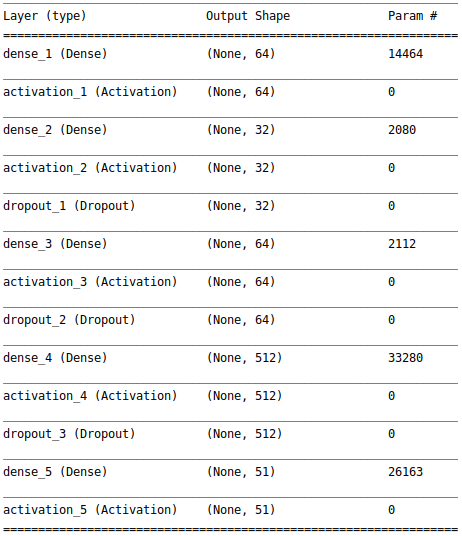
\includegraphics[width=.85\textwidth]{img/keras_network_summary.png}
			\end{center}
		\end{column}		
	\end{columns}
\end{frame}

\begin{frame}[t]{Klassifizierung mit Tensorflow - Erste Ergebnisse}
	\begin{columns}
		\begin{column}[t]{6cm}
			\begin{center}
			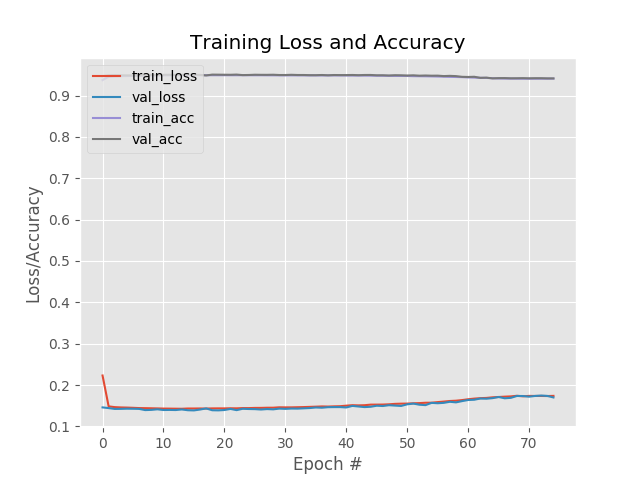
\includegraphics[width=1\textwidth]{img/keras_training_loss.png}
			\end{center}
		\end{column}
		\begin{column}[t]{6cm}

		\end{column}		
	\end{columns}
\end{frame}

\begin{frame}[t]{Klassifizierung mit Tensorflow - Erste Ergebnisse}
	\begin{columns}
		\begin{column}[t]{6cm}
			\begin{center}
				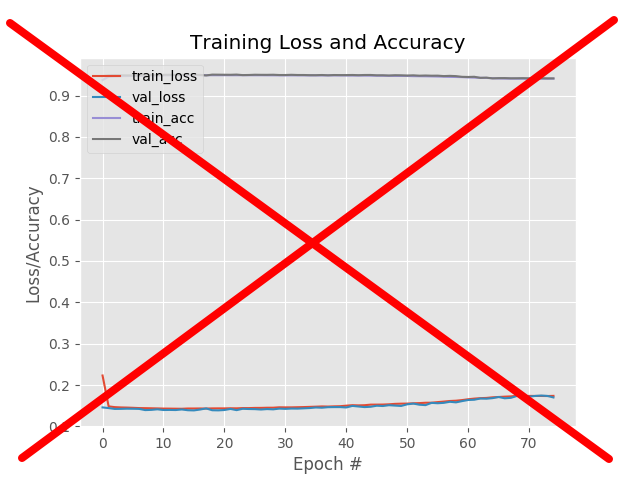
\includegraphics[width=1\textwidth]{img/keras_training_loss_invalid.png}
			\end{center}
		\end{column}
		\begin{column}[t]{6cm}
			\begin{itemize}
				\item Manuelle Verifikation deutet wesentlich schlechtere Resultate an
				\item Erste Klassifizierung möglich
			\end{itemize}
			\vspace*{20px}
Probleme:
			\begin{itemize}
				\item Gewichtung der NaN-Labels 
			\end{itemize}
		\end{column}		
	\end{columns}
\end{frame}

\begin{frame}[t]{Klassifizierung mit Tensorflow - Nächste Schritte}
	\begin{itemize}
		\item Finden einer geeigneten Verlustfunktion
		\item Multi-Label-Evaluation
		\item Verwenden von Gewichten
	\end{itemize}
\end{frame}

\begin{frame}[t]{Klassifizierung mit XGBoost}
	\begin{itemize}
		\item Bibliothek für GPU-unterstützte und verteilte Berechnung von \emph{Gradient Boosted Trees}
	\end{itemize}
	Vorteile:
	\begin{itemize}
		\item liefert gute Ergebnisse für tabulare Daten
		\item Scikit-learn API vorhanden $\rightarrow$ Verwendung der Scikit-learn Infrastruktur problemlos möglich, insbesondere \emph{OneVsRestClassifier}
		\item gute Interpretierbarkeit $\rightarrow$ Bibliothek kann berechnete Bäume und \emph{Feature Importances} als Plots ausgeben
	\end{itemize}
	Nachteile:
	\begin{itemize}
		\item hoher Berechnungsaufwand, insbesondere für Multilabel-Klassifizierung (Training von 51 Modellen)
		\item Hyperparametersuche schwierig
	\end{itemize}
\end{frame}

\begin{frame}[t]{Hyperparametertuning mit Bayesian Optimization}
	\begin{itemize}
		\item Training auf ganzem Datensatz dauert zu lange und ist auf GPU nicht möglich $\rightarrow$ für Hyperparametersuche Beschränkung auf jeweils fünf zufällig gewählte Attribute
		\item Suche guter Startpunkte für Hyperparameter mit \emph{Randomized Search CV}
		\item Verfeinerung der Parameter mit \emph{Bayesian Optimization}
		\begin{itemize}
			\item Maximierung einer unbekannten Funktion durch Interpolation dieser anhand bekannter Startwerte und statistisch sinnvoll gewählten weiteren Parametersätzen
		\end{itemize}
		\item Mögliches Problem: optimale Hyperparameter unterscheiden ggf. sich für verschiedene Label
	\end{itemize}
\end{frame}

\section{Probleme und offene Fragen}

\begin{frame}[t]{Learning Rate und N\_Estimators}
	\begin{itemize}
		\item letzte Boosting-Runde in der Regel nicht die beste $\rightarrow$ verwende \emph{Early Stopping}
		\item Parameterempfehlung für \emph{Learning Rate}: $2 \text{ bis } 10 \div \operatorname{n\_estimators}$
		\item Problem bei uns: beste Iteration ist immer die letzte, auch bei deutlich höheren Lernraten
	\end{itemize}
\end{frame}

\begin{frame}[t]{NaN-Werte in den Labeln}
	\begin{itemize}
		\item viele der Label des Datensatzes sind weder True noch False, sondern NaN (also fehlend)
		\item wir setzen fehlende Label aktuell auf False $\rightarrow$ Problem wird durch einige falsche Label schwerer
		\item in Vaizman et al. (2017) wurden NaN-Label bei Training und Testen ignoriert - wir sollen vermutlich genauso vorgehen?
	\end{itemize}
\end{frame}

\begin{frame}[t]{Aufteilung Trainings- und Testdaten}
	\begin{itemize}
		\item Vaizman et al. teilen die Trainings- und Testdaten auf Basis der einzelnen Benutzer auf $\rightarrow$ beim Testen werden nur Daten von zuvor unbekannten Personen betrachtet
		\item andere Möglichkeit: zufällige Aufteilung aller Daten von allen Personen $\rightarrow$ deutlich leichteres Problem
		\item Frage: welche Aufgabe sollen wir genau lösen?
	\end{itemize}
\end{frame}

\section{Pläne für die Zukunft}

\begin{frame}[t]{Pläne und Ideen}
	\begin{itemize}
		\item Verwendung der bisherigen Classifier und spätere Entscheidung welcher besser funktioniert
		\item Aufbereitung des Datensatzes
		\begin{itemize}
			\item \emph{Maximal Correlation Embeddings} [Li et al. 19], um fehlende Label in den Trainingsdaten zu ersetzen
			\item Rekonstruktion fehlender Sensordaten mit einem \emph{Adversarial Autoencoder} [Saeed et al. 18]
		\end{itemize}
		\item Auslesen der \emph{Feature Importances} und Entscheidungsbäume pro Label bei XGBoost (jeweils 51 Stück)
	\end{itemize}
\end{frame}

\end{document}
